\documentclass[a4paper, 12pt]{article}
\usepackage{titling}
\usepackage{array}
\usepackage{booktabs}
\usepackage{enumitem}
\usepackage{graphicx}
\usepackage{hyperref}
\usepackage{amssymb}
\usepackage{color}
\usepackage{listings}
\setlength{\heavyrulewidth}{1.5pt}
\setlength{\abovetopsep}{4pt}
\setlength{\parindent}{0pt}
\graphicspath{{.}}

\usepackage[margin=1in]{geometry}

% Must be after geometry
\usepackage{fancyhdr}
\pagestyle{fancy}
\fancyhf{}
\rhead{SEE Assignment 3}
\lhead{P.Lukin, E. Ovchinnikova}
\cfoot{\thepage}

\setlength{\droptitle}{-5em}

\title{Scientific Experimentation and Evaluation  \\
				Assignment: 2.1}
\author{Petr Lukin, Evgeniya Ovchinnikova}
\date{Lecture date: $10^{th}$ October 2016}

\begin{document}



\maketitle

\section{Calibration setup}

In this work we are using photogrammetric method for camera calibration ~\cite{1}. \\ First step of the calibration is to connect camera to laptop and test if it can capture still picture. Camera was connected to a laptop with Fedora operation system. A default program for USB cameras (Cheese) couldn't perform automatic brightness adjustment and the camera picture was almost white, so we decided on usage GUVCView that provides a very nice GUI that allows to easily adjust such important parameters as brightness, contrast, resolution, etc. (Fig.\ref{fig:guvcview}).

\begin{figure}[h]
  \centering
  \caption{GUVCView GUI.\label{fig:guvcview}}
  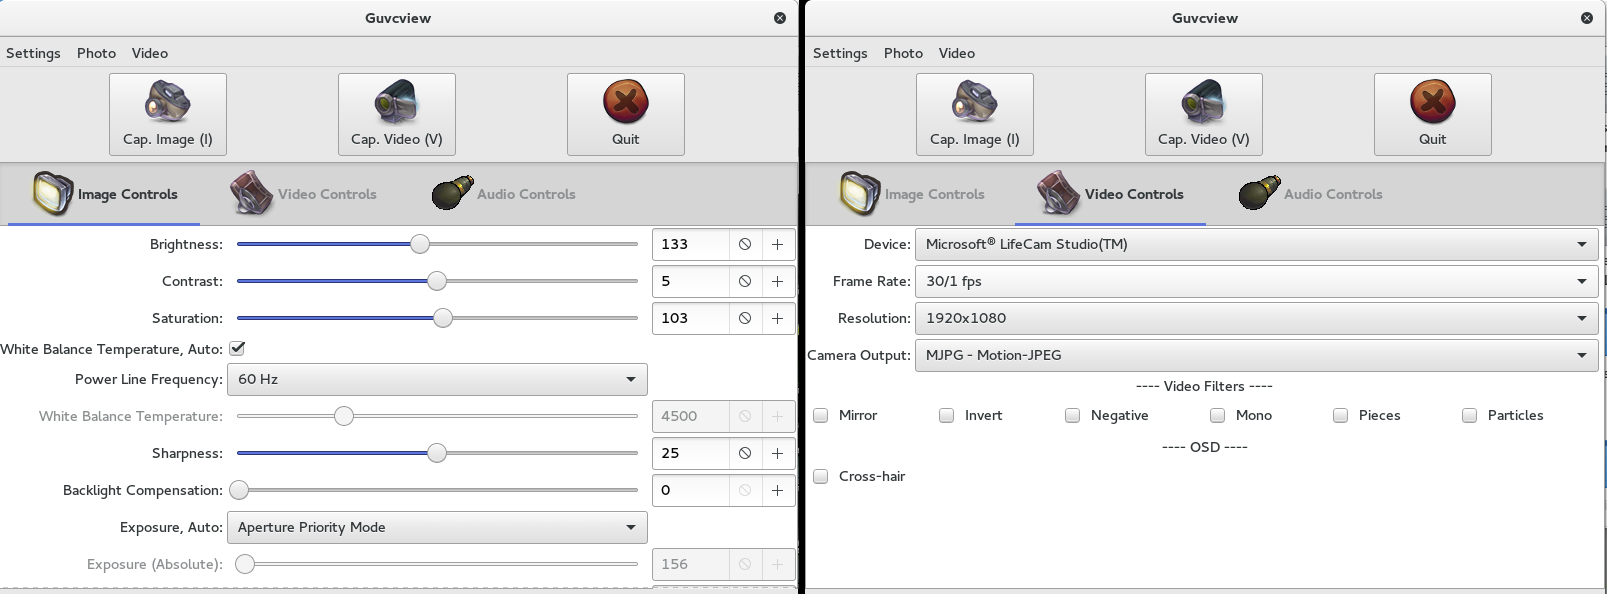
\includegraphics[width=1.0\textwidth]{guvcview}
\end{figure}

Next step is to install the camera on the tripod to fix the camera's position. Tripod was meant for another type of camera, however, it can be fixated by clamping. Camera on the tripod is depicted in Fig. \ref{fig:tripod}. 

\begin{figure}[h]
  \centering
  \caption{Camera on tripod.\label{fig:tripod}}
  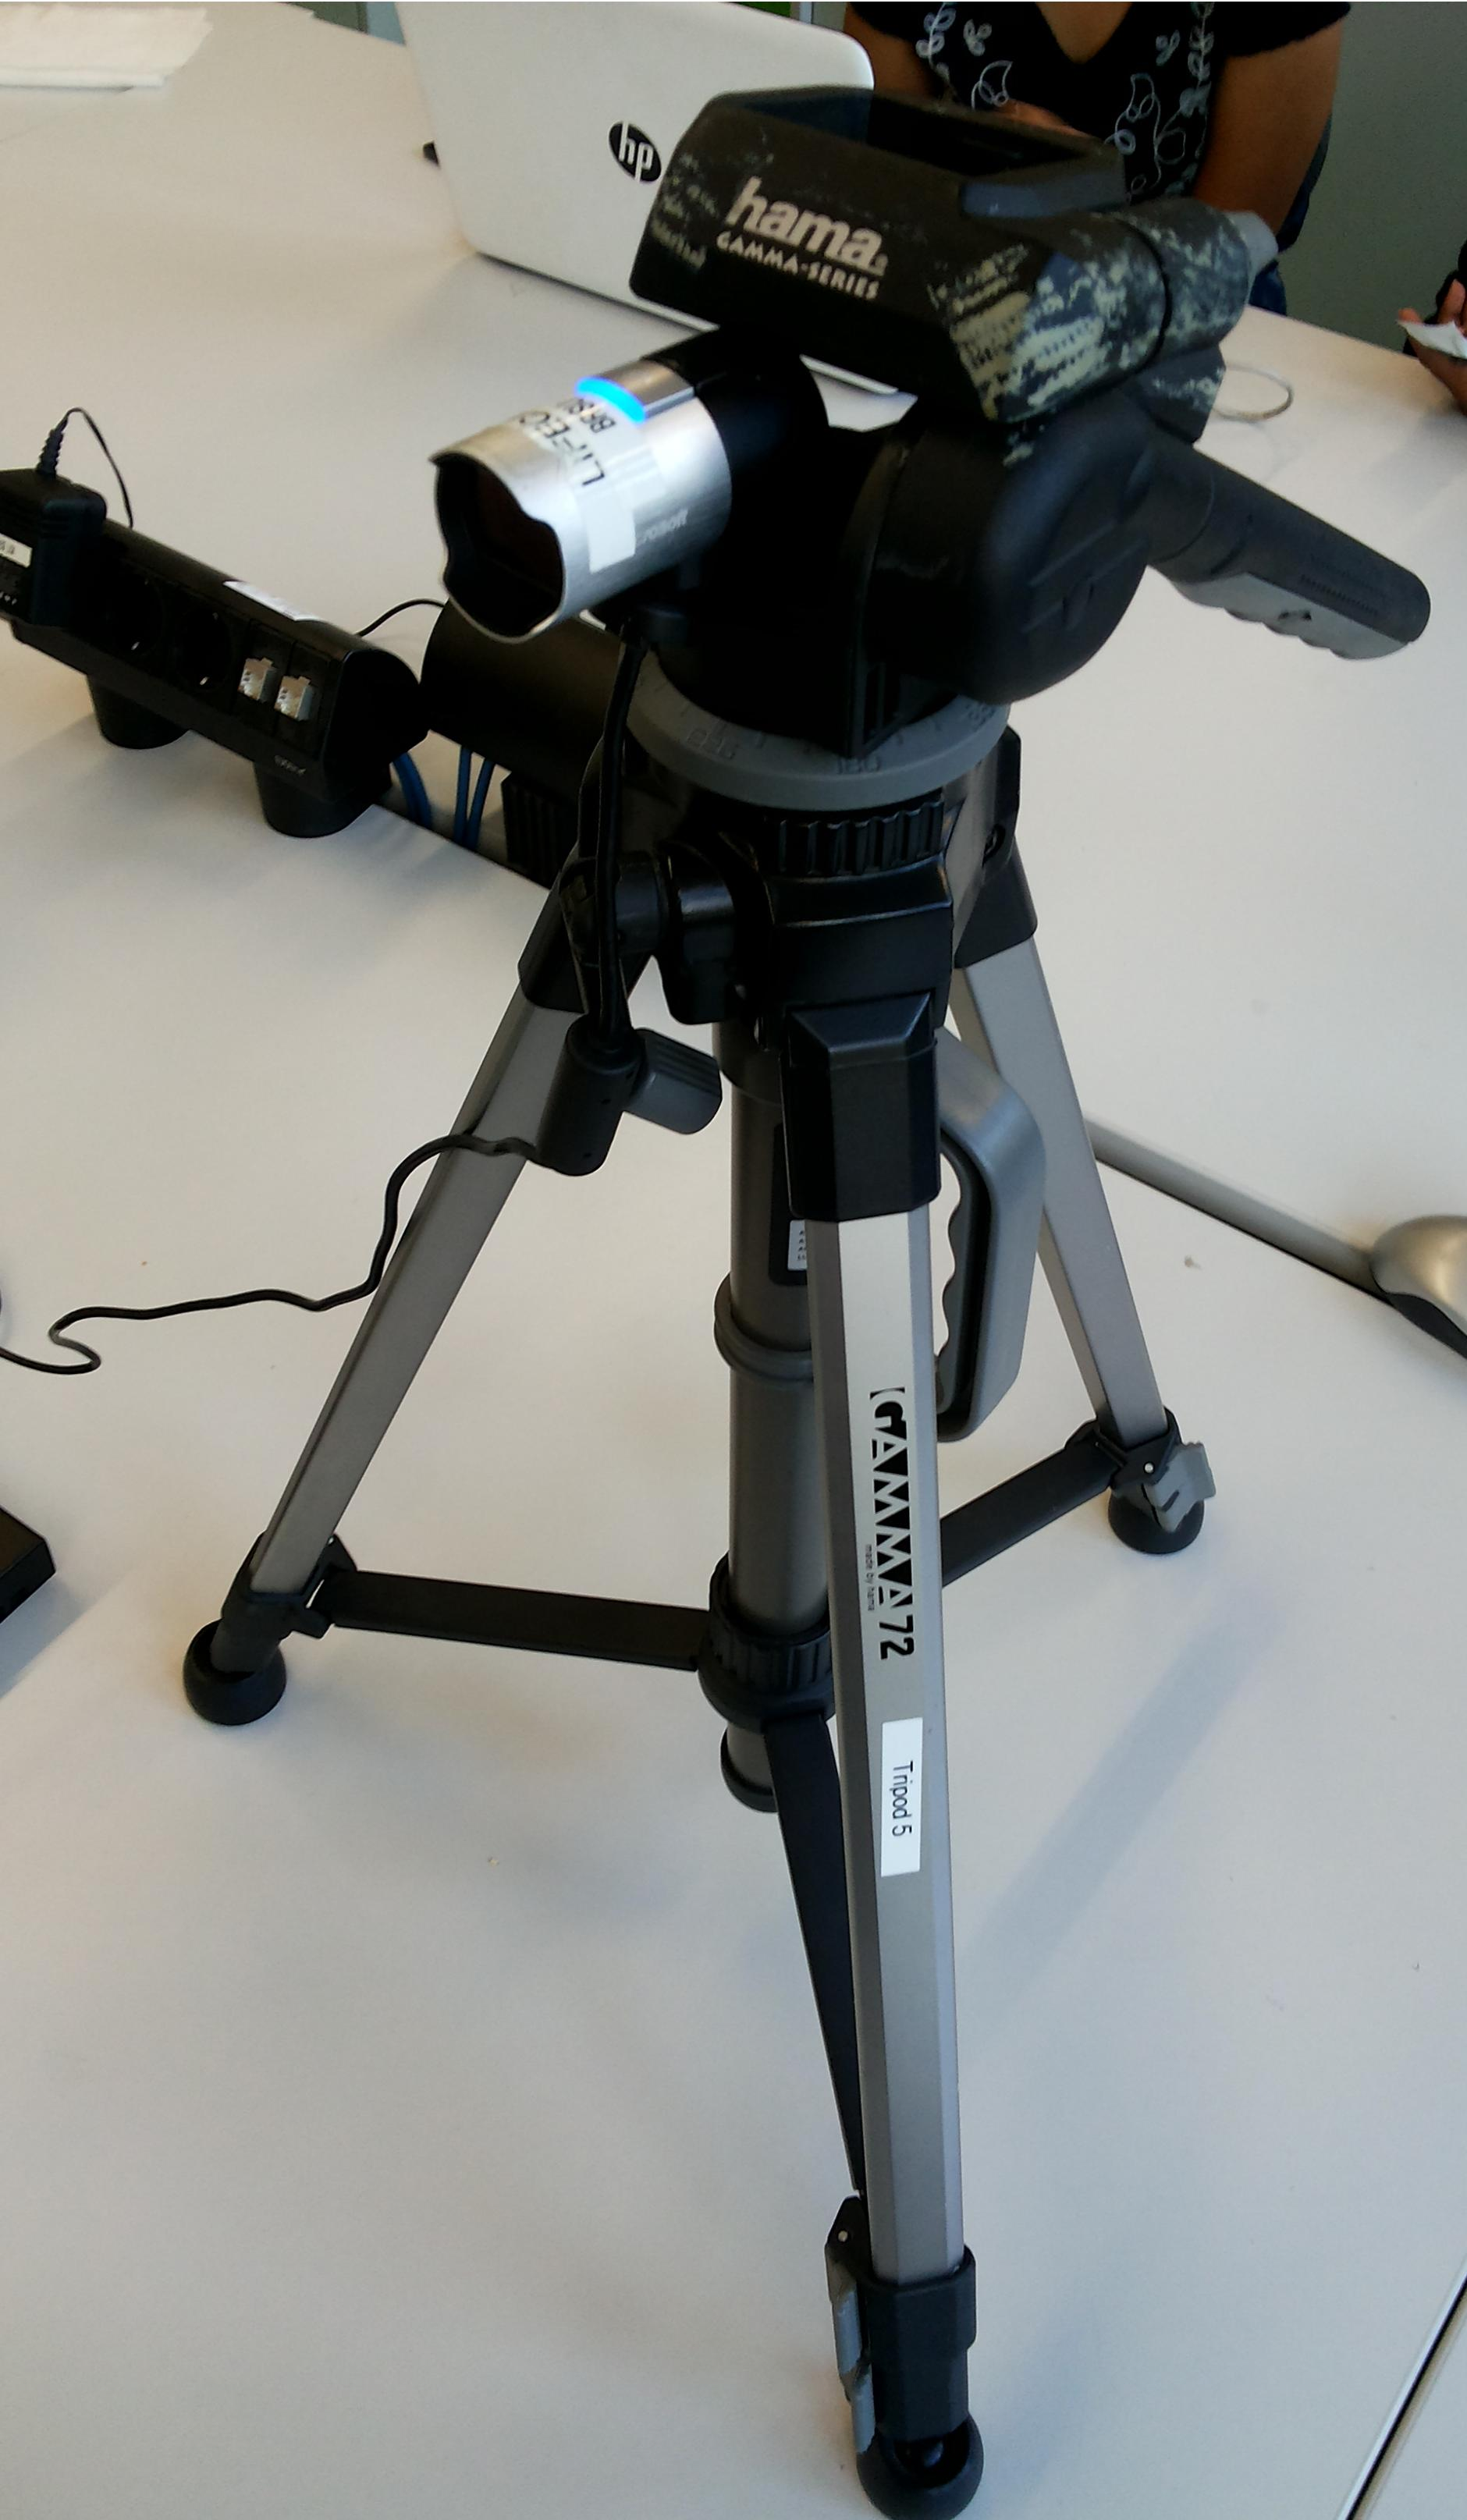
\includegraphics[width=0.5\textwidth]{tripod}
\end{figure}

For calibration we have chosen a large "chessboard" with 72mm square side from room C022 (Fig. \ref{fig:chessboard}) and a standard Matlab calibration application. 

\begin{figure}[h]
  \centering
  \caption{Calibration "chessboard".\label{fig:chessboard}}
  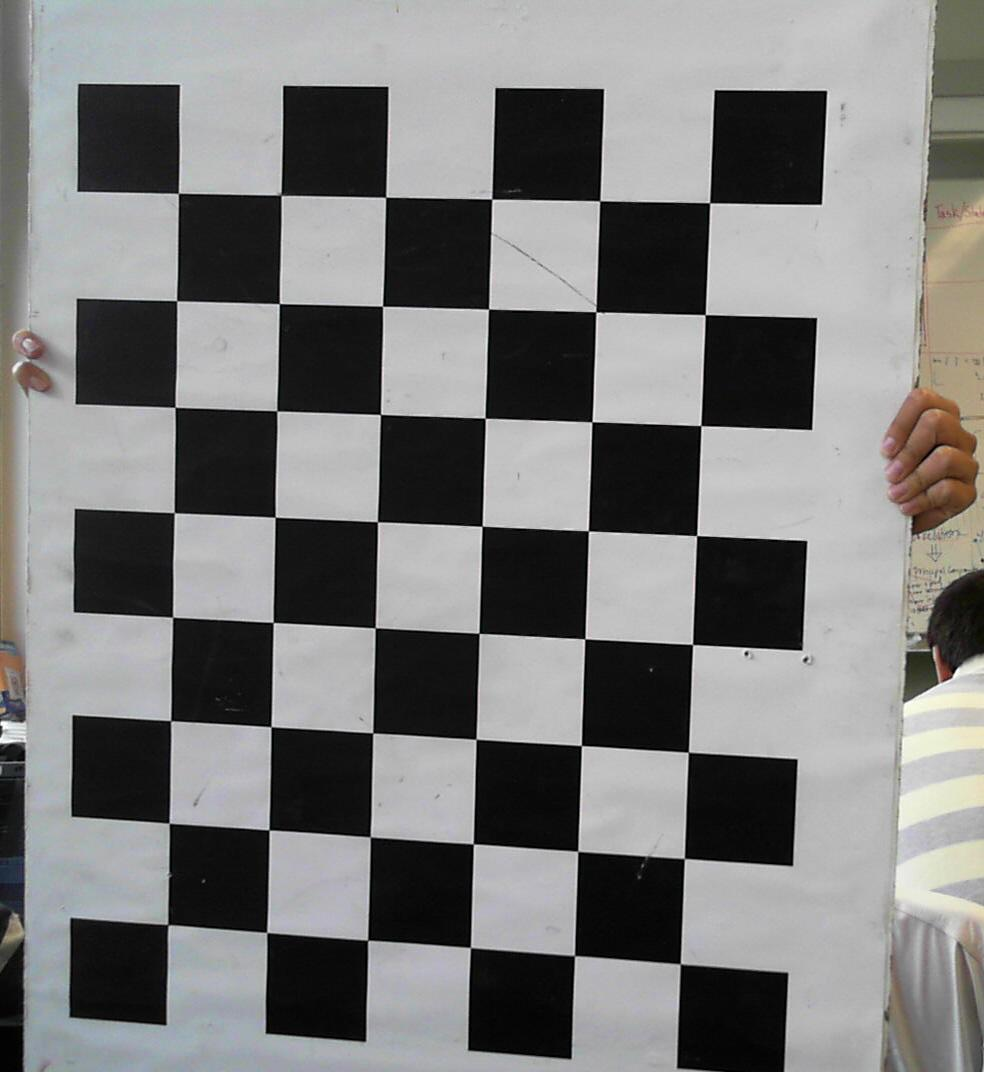
\includegraphics[width=0.5\textwidth]{chessboard}
\end{figure}

There are the following possible pitfalls of the calibration:
\begin{itemize}
\item since the "chessboard" is heavy, it was hard to hold it straight, especially under some angles, so the pictures could be a bit blurred
\item some pictures were taken with different lighting that could affect the quality of the pictures
\item some pictures (one in our case) are not accepted by the calibration tool
\item calibration board can have some irregularity
\item we are using such a camera model that doesn't use the skew, so if there is the one, it may cause the problems
\item imperfections of the camera
\end{itemize}


\section{Experiment}

We've captured the images of the "chessboard" under different angles (Fig. \ref{fig:positions}, first line) and in different positions in the camera frame (Fig. \ref{fig:positions}, second line), so we would have a better coverage of a camera matrix. The number of pictures was chosen experimentally, based on the look of undistorted picture. First we've used around 20 pictures with different angles of chessboard, but not covering the camera frame enough and obtained an image depicted in Fig. \ref{fig:distort} that is obviously bad-calibrated. Therefore we have added another 10 pictures those cover sides of the camera frame and obtained a well undistorted picture (Fig. \ref{fig:undist}).

\begin{figure}[h]
  \centering
  \caption{"Chessboard's" positions.\label{fig:positions}}
  \includegraphics[width=1.0\textwidth]{positions}
\end{figure}

\begin{figure}[h]
  \centering
  \caption{Example of a bad calibration.\label{fig:distort}}
  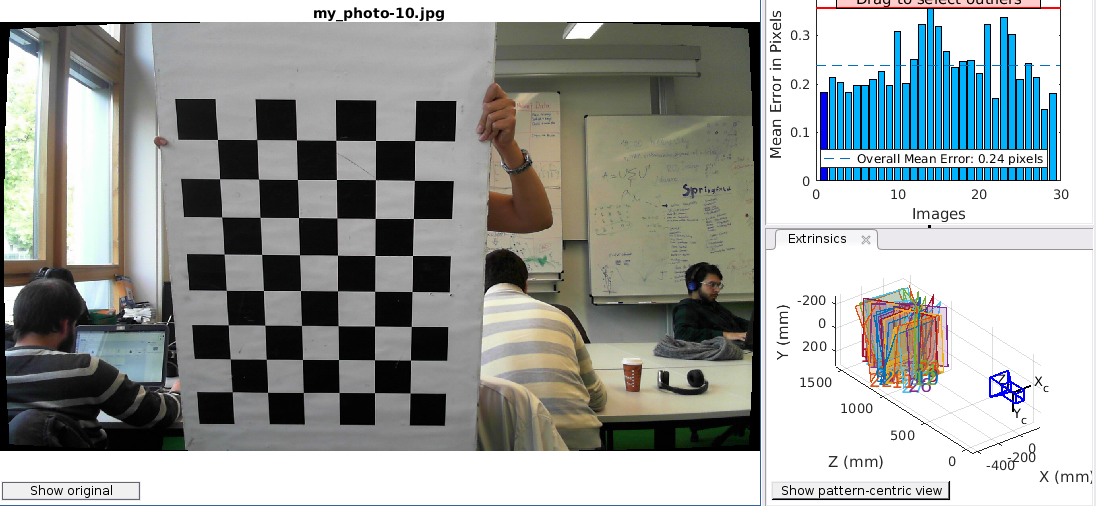
\includegraphics[width=1.0\textwidth]{distort}
\end{figure}


\begin{figure}[h]
  \centering
  \caption{Well-undistorted picture.\label{fig:undist}}
  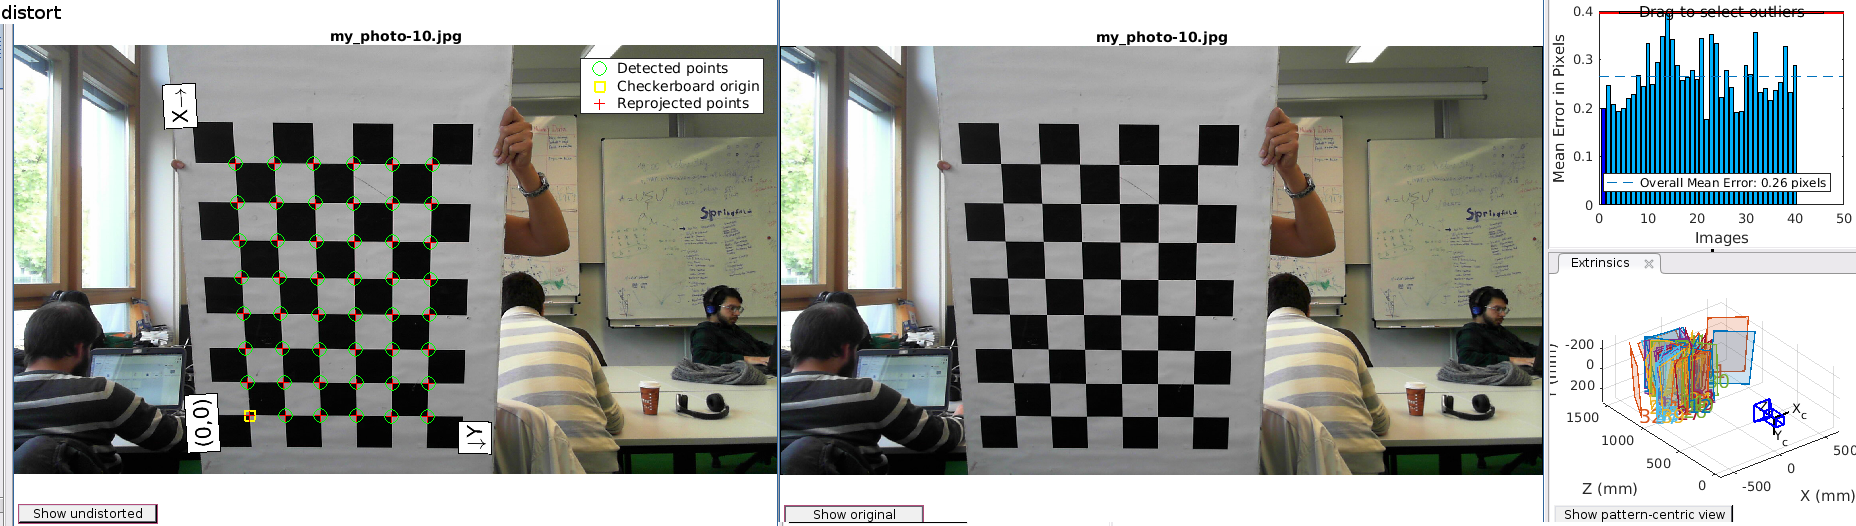
\includegraphics[width=1.0\textwidth]{undist}
\end{figure}

The following script was used for calibration:

\begin{lstlisting}
% Auto-generated by cameraCalibrator app on 16-Oct-2016
%-------------------------------------------------------


% Define images to process
imageFileNames = 
{'/home/elhe/Uni/WS2016/SEE/Assignments/20161010/my_photo-10.jpg',...
...
    '/home/elhe/Uni/WS2016/SEE/Assignments/20161010/my_photo.jpg',...
    };

% Detect checkerboards in images
[imagePoints, boardSize, imagesUsed] = 
detectCheckerboardPoints(imageFileNames);
imageFileNames = imageFileNames(imagesUsed);

% Generate world coordinates of the corners of the squares
squareSize = 72;  % in units of 'mm'
worldPoints = generateCheckerboardPoints(boardSize, squareSize);

% Calibrate the camera
[cameraParams, imagesUsed, estimationErrors] =
	 estimateCameraParameters(imagePoints, worldPoints, ...
    'EstimateSkew', false, 'EstimateTangentialDistortion', false, ...
    'NumRadialDistortionCoefficients', 2, 'WorldUnits', 'mm', ...
    'InitialIntrinsicMatrix', [], 'InitialRadialDistortion', []);

% View reprojection errors
h1=figure; showReprojectionErrors(cameraParams, 'BarGraph');

% Visualize pattern locations
h2=figure; showExtrinsics(cameraParams, 'CameraCentric');

% Display parameter estimation errors
displayErrors(estimationErrors, cameraParams);

% For example, you can use the calibration data to
remove effects of lens distortion.
originalImage = imread(imageFileNames{1});
undistortedImage = undistortImage(originalImage, cameraParams);


\end{lstlisting}	

\section{Experimental results}

After the calibration we have obtained the following results:

\begin{lstlisting}

cameraParams = 

  cameraParameters with properties:

   Camera Intrinsics
                    IntrinsicMatrix: [3x3 double]
                        FocalLength: [1.4510e+03 1.4511e+03]
                     PrincipalPoint: [968.9125 552.0061]
                               Skew: 0

   Lens Distortion
                   RadialDistortion: [0.0024 0.0017]
               TangentialDistortion: [0 0]

   Accuracy of Estimation
              MeanReprojectionError: 0.2644
                 ReprojectionErrors: [48x2x40 double]
                  ReprojectedPoints: [48x2x40 double]

   Calibration Settings
                        NumPatterns: 40
                        WorldPoints: [48x2 double]
                         WorldUnits: 'mm'
                       EstimateSkew: 0
    NumRadialDistortionCoefficients: 2
       EstimateTangentialDistortion: 0

\end{lstlisting}

Here skew and tangential distortion are zero because of the chosen model. The  intrinsic matrix is parameterized as the following ~\cite{2}:\\
\[ \left( \begin{array}{ccc}
f_x & s & x_0 \\
0 & f_y & y_0 \\
0 & 0 & 1 \end{array} \right)\],
where each parameter is a geometrical parameter of the camera. $f_x, f_y$ are focal lengths those for a perfectly spherical camera are equal (Fig. \ref{fig:focal}). In our case they are slightly different. It could be caused by imperfectance of the camera, non-uniformed scaling of the pictures or calibrations errors. However, difference is small enough to use this calibration in further work.



\begin{figure}[h]
  \centering
  \caption{Focal length ~\cite{2}.\label{fig:focal}}
  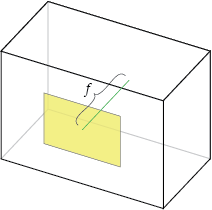
\includegraphics[width=0.3\textwidth]{focal}
\end{figure}

$x_0, y_0$ is principal point offset that shows the coordinates of the printipal point relatively to the principal axis (Fig. \ref{fig:principal}).

\begin{figure}[h]
  \centering
  \caption{Principal axis and principal poin. ~\cite{2}.\label{fig:principal}}
  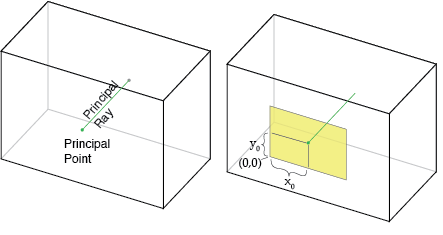
\includegraphics[width=0.5\textwidth]{principal}
\end{figure}

Radial distortion is small that shows that the calibration was quite successful and mean reprojection error confirms it, because it is less than 0.5 pixels.

\begin{thebibliography}{3}
\bibitem{1}
Zhang, Z. 2000. A flexible new technique for camera calibration. IEEE TPAMI, 22(11):1330–1334.
\bibitem{2}
\url{http://ksimek.github.io/2013/08/13/intrinsic/}

\end{thebibliography}




\end{document}
